%  1)  latex  aipsamp
%  2)  bibtex aipsamp
%  3)  latex  aipsamp
%  4)  latex  aipsamp
\pdfinclusioncopyfonts=1
\documentclass[%
 aip,
% jmp,
% bmf,
% sd,
% rsi,
 amsmath,amssymb,
preprint,%
% reprint,%
%author-year,%
author-numerical,%
% Conference Proceedings
]{revtex4-1}
\usepackage{graphicx}% Include figure files
\usepackage{dcolumn}% Align table columns on decimal point
\usepackage{bm}% bold math
\usepackage[mathlines]{lineno}% Enable numbering of text and display math
\linenumbers\relax % Commence numbering lines
\usepackage[utf8]{inputenc}
\usepackage[T1]{fontenc}
\usepackage{mathptmx}
\usepackage{amsmath}
\usepackage{amssymb}
\usepackage{amsfonts}
\usepackage{color} 

\begin{document}

\preprint{AIP/123-QED}

\title[LLJ \& shear]{Effect of turbine-height on wind farm performance in the presence of a low-level jet}

\author{Srinidhi N. Gadde}
 \email{s.nagaradagadde@utwente.nl}
%Lines break automatically or can be forced with \\
\author{Richard J. A. M. Stevens}%
\affiliation{Physics of Fluids Group, Max Planck Center Twente for Complex Fluid Dynamics, J. M. Burgers Center for Fluid Dynamics and MESA+ Research Institute, University of Twente, P. O. Box 217, 7500 AE Enschede, The Netherlands}

\date{\today}% It is always \today, today,
             %  but any date may be explicitly specified

\begin{abstract}
Low-level jets (LLJs) are the wind maxima in lowest 50-1000 m of the stable atmospheric boundary layers. Due to their significant influence on the power production of wind farms, it is crucial to understand the interaction between LLJs and wind farms. In the presence of an LLJ, there are positive and negative shear regions in the velocity profile. Furthermore, the positive shear regions of LLJs are continuously turbulent, while the negative shear regions have limited turbulence. We present large eddy simulations of wind farms in which we vary the height of the wind turbines such that the turbine rotor area is either completely or partially immersed in the positive and negative shear region of the jet. We find that the wakes recover relatively fast when the turbines are below the jet. In this case, most energy from the LLJ is harvested by the first rows of the wind farm due to strong downward vertical entrainment induced by the wakes. However, when the height of the turbines extends into the negative shear region of the boundary layer, the wake recovery behind the first rows of the wind farm is very slow due to the low atmospheric turbulence above the top of surface inversion. When the turbine rotor area is equally distributed between above and below the jet, the entrainment fluxes are minimal. However, when the turbine rotor area is completely above the jet, we find that positive entrainment fluxes generated by the negative shear facilitate energy extraction from the jet further downstream in the wind farm and slightly improves power production.
\end{abstract}
\keywords{Low-level jet; Wind farm; Large eddy simulation; Stable boundary layer; Shear}

\maketitle

\section{Introduction}\label{sec1}


The atmospheric boundary layer (ABL) forms the lowest part of the atmosphere, where the effects of friction due to the surface of the Earth are prominent. The ABL continuously undergoes transition due to the changes in the radiative heat transfer at the ground and the geostrophic wind. When the ABL transitions from neutral to stable due to surface cooling, the wind above the surface layer is decoupled from surface friction. Consequently, the balance between the {\color{black}pressure, the Coriolis, and the frictional forces is altered, and} the flow above the surface layer accelerates. When such a wind is subjected to inertial oscillations it reaches super-geostrophic magnitudes and forms a LLJ. These jets are observed in the lowest 50 to 1000 m of the ABL \citep{sme96} and are most pronounced in weak to moderately stable ABLs \cite{baa09, ban08}. Such LLJs \cite{kel04, ban02, sme93} have been reported all over the world with frequent occurrences in India \cite{pra11}, China \cite{liu14}, the Great Plains of the United States \cite{arr97} and the North Sea region of Europe \cite{kal19, wag19}. North Sea LLJs have been studied extensively in field observations \cite{kal17, dun18} and using mesoscale models \cite{kal19}. Field observations show that near IJmuiden, the frequency of occurrence of the LLJ is 7.56\% in summer and 6.61\% during the spring. LLJs in the North Sea have been associated with very low boundary-layer heights, around 50-120 m \cite{dun18}. As a result, the importance, relevance, and urgency of studying LLJ for wind farm applications have been outlined by van Kuik et al.\ \cite{kui16} in their long term European Research Agenda and a recent review by Port\'e-Agel et al.\ \cite{por20}. Figure \ref{fig1} shows a sketch of the stably stratified LLJ velocity profile with corresponding temperature and turbulence flux profiles.\\
%Due to their importance LLJ characteristics have been studied in classical works such as Mahrt \cite{mah99}, Poulos et al.\ \cite{pou02}, and Beare et al.\ \cite{bea06}.
%The GABLS-1 (Global Earth and Water Cycle Experiment Atmospheric Boundary Layer study-1) stable boundary layer is a widely recognized benchmark case designed to study stable boundary layer dynamics. Therefore, previous studies have been used to study the effect of LLJs on wind turbines and wind farms \cite{wu11, bha14, bha15, na18}.
\indent It is well established in the wind energy community that the presence of LLJs can affect the performance of wind turbines \cite{sis78}. Below the jet height $z_\mathsf{jet}$ the velocity profile has a positive shear, and above the jet height there is a negative shear. The schematic in Fig.\ \ref{fig1} shows the corresponding possible scenarios. The top panel of Fig.\ \ref{fig1} shows a turbine with the hub-height $z_h$ lower than the jet height, i.e.\ $z_h < z_\mathsf{jet}$, operating in the positive shear region. The bottom panel shows a turbine with the hub-height higher than the jet height, i.e.\ $z_h > z_\mathsf{jet}$, operating in the negative shear region. Due to the velocity maximum and strong shear, both the power production and the fatigue loads on wind turbines are affected by the LLJ \cite{gut17}. It has been reported that LLJs can increase the capacity factors by 60\% under nocturnal conditions \cite{wil15b} and measurements in Western Oklahoma\cite{gre09} indicate that LLJs increase the power production compared to the case without jets.\\
\indent LLJs generally form at the stable surface inversions \cite{baa09}, above which the turbulence is negligible \cite{bla57}. {\color{black} Therefore, performance of wind farms under different thermal stratification i.e. stable, unstable, and diurnal conditions has been previously studied in the literature \cite{dor15, abk16, ali18b, ali19, all18}.} {\color{black}It has been reported that during an LLJ event the turbulence intensity and turbulence kinetic energy are lower than for unstable conditions \cite{gut16}.} The effect of LLJs on wind turbine and wind farm performance has been studied before. Lu \& Port{\'e}-Agel \cite{lu11} performed large eddy simulations (LES) of an `infinite' windfarm in the GABLS-1 stable boundary layer and they report the formation of non-axisymmetric wakes and a decrease in the LLJ strength due to the energy extraction by the turbines. {\color{black}LLJ elimination due to wind turbine momentum extraction has also been reported in similar LES studies \cite{abk16, bha15, sha17d, ali17}.} Also, mesoscale simulations in which wind farms are modeled as localized roughness elements, show that LLJs are eliminated by wind farms\cite{fit13}.

\begin{figure}
 \centering
 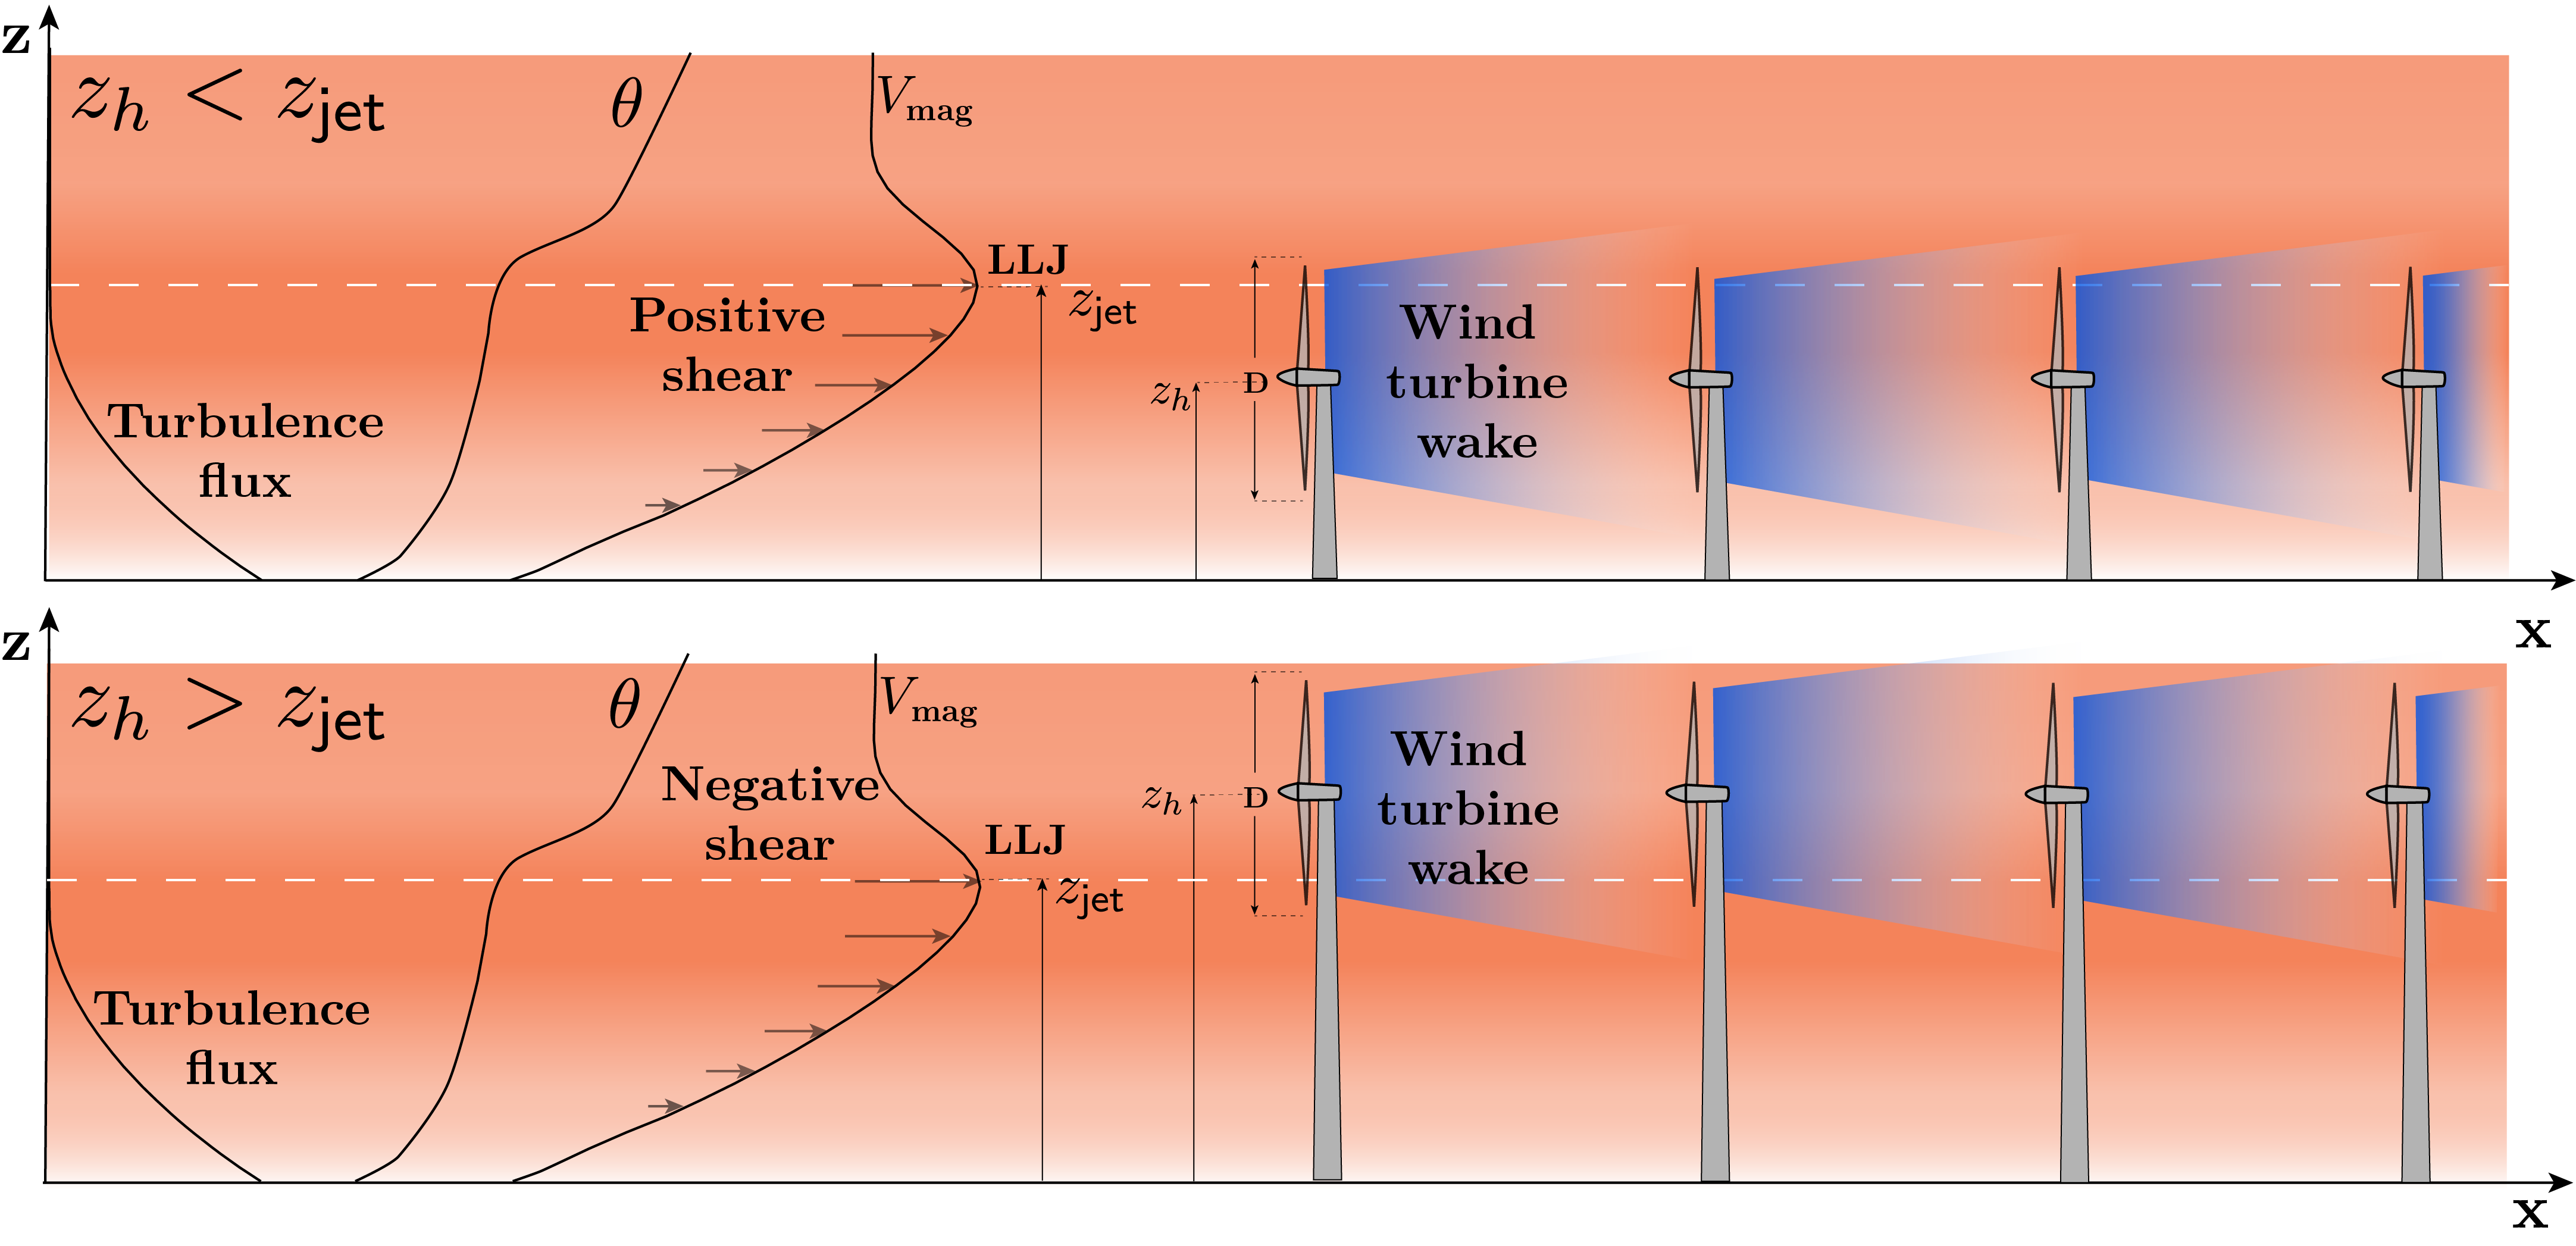
\includegraphics[width=1.0\linewidth]{llj_2.png}
 \vspace{-0.5cm}
 \caption{Schematic showing different scenarios in a wind farm in the presence of a LLJ and temperature inversion. Both positive and negative shear regions are indicated. The top figure shows turbines operating in positive shear (turbine hub-height is below the jet height i.e.\ $z_h < z_\mathsf{jet}$), and the bottom figure shows turbines operating in negative shear (turbine hub-height is above the jet height i.e.\ $z_h > z_\mathsf{jet}$). The flow is continuously turbulent below the jet-height and has negligible turbulence above.}
 \label{fig1}
\end{figure}

In a fully developed wind farm boundary layer the power production depends on the vertical entrainment fluxes from above created by the momentum deficit inside the wind farm. Wind turbines operating below the LLJ are subjected to positive shear and continuous turbulence. In that case the vertical entrainment fluxes are enhanced due to which the energy of the LLJ is harvested by the first couple of turbine rows \cite{na18, nag20b}. However, modern wind turbines are reaching heights above $200$ m at which the interaction with LLJs is inevitable and situations might arise when the turbines have to operate in the negative shear region with reduced turbulence. Aeroelastic simulations of the interaction between an LLJ and a wind turbine show that the loading on the wind turbines decreases when they operate in the jet's negative shear region. Based on these simulations, Gutierrez et al.\ \cite{gut17} suggest installing turbines at heights where negative shear occurs. They report that negative shear reduces the structural damage associated with positive shear and aids in capturing LLJ energy. However, the region where negative shears occur is also a region of reduced turbulence. Wake recovery behind the turbines operating in a turbulent region is generally higher than the wake recovery behind a turbine operating in a non-turbulent atmosphere \cite{ste17, por20, ali18b}. However, higher stability in the region of negative shear might also affect the wake recovery and hence power production.

Previous studies have mostly focused on wind turbines and wind farms operating in the positive shear region of the jet. However, as turbine heights increase it is important to investigate what happens when turbines operate above the jet, i.e.\ in the negative shear region. The presence of negative shear and low-boundary layer height leads to scenarios in which a wind farm and LLJ interaction are not straightforward. By performing LES of a large wind farm we study the effect of negative shear of a LLJ on the performance of a wind farm. This is important to better understand the coupling between the wind farm turbulence and LLJ shear on wind farm power production. As the GABLS-1 stable boundary layer benchmark case is ideal for studying the physical phenomena that emerge when LLJs interact with a large wind farm we use in this study. We consider three LES corresponding to the following scenarios:
\vspace{-2.5mm}
\begin{itemize}
\item[1.] The turbine hub-height is below the jet height and the rotor area is completely below the jet, i.e.\ $z_h < z_\mathsf{jet}$.
\vspace{-2.5mm}
\item[2.] The turbine hub-height is equal to the jet height and rotor area is equally distributed above and below the jet, i.e.\ $z_h \approx z_\mathsf{jet}$.
\vspace{-2.5mm}
\item[3.] The turbine hub-height is above the jet height and rotor area is completely above the jet, i.e.\ $z_h > z_\mathsf{jet}$.
\end{itemize}
%%%%%%%%%%%%%%%%%%%%%%%%%%%%%%%%%%%%%%%%%%%%
In section \ref{sec2} the simulation methodology and the wind farm configuration are described. In section \ref{sec3} the main observations are discussed and in section \ref{sec4} the major conclusions are detailed. 

%%%%%%%%%%%%%%%% Section 2 %%%%%%%%%%%%%%%%%%%%%%%%%%
\section{Simulation methodology}\label{sec2}

\subsection{Governing equations}\label{sec2.1}
We numerically integrate the filtered Navier-Stokes equation coupled with the Boussinesq approximation to model buoyancy. The governing equations are: 
%
\begin{align}
 \partial_{\mathit{i}} \widetilde{u}_\mathit{i}&=0,\label{eqn1}\\
 \begin{split}
 \partial_{\mathit{t}}\widetilde{u}_\mathit{i} + \partial_\mathit{j}\left(\widetilde{u}_\mathit{i}\widetilde{u}_\mathit{j}\right)&=-\partial_{\mathit{i}}\widetilde{p}-\partial_\mathit{j}\tau_{\mathit{ij}} + g\beta(\widetilde{\theta}-\widetilde{\theta}_\mathit{0})\delta_{\mathit{i3}}+f_c(U_g-\widetilde{u})\delta_{i2}-f_c(V_g-\widetilde{v})\delta_{i1}+ \widetilde{f}_x\delta_{i1}+ \widetilde{f}_y\delta_{i2},
 \end{split}\label{eqn2}\\
 \partial_{\mathit{t}}\widetilde{\theta} + \widetilde{u}_\mathit{j}\partial_{\mathit{j}}\widetilde{\theta}&=-\partial_{\mathit{j}}q_\mathit{j},\label{eqn3}
\end{align}
%
here the tilde represents a spectral cut-off filter of size $\Delta$, $\widetilde{u}_\mathit{i}=\left(\widetilde{u},\widetilde{v},\widetilde{w}\right)$ and $\widetilde{\theta}$ are the filtered velocity and potential temperature, respectively, $g$ is the gravitational acceleration, $\beta=1/\theta_\mathit{0}$ is the buoyancy parameter with respect to the reference potential temperature $\theta_\mathit{0}$, $\delta_{\mathit{ij}}$ is the Kronecker delta, and $f_c$ is the Coriolis parameter. The ABL is forced by a mean pressure $p_\infty$, represented by the geostrophic wind with the relation, $U_g=-\frac{1}{{\rho}f_c}\frac{\partial{p_{\infty}}}{\partial{y}}$ and $V_g=\frac{1}{{\rho}f_c}\frac{\partial{p_{\infty}}}{\partial{x}}$ as its components. $\widetilde{p}=\widetilde{p}^{*}/\rho+\sigma_{kk}/3$ is the modified pressure, which is the sum of the trace of the SGS stress, $\sigma_{kk}/3$, and the kinematic pressure $\widetilde{p}^{*}/\rho$, where $\rho$ is the density of the fluid. 

It is well established that the actuator disk model can capture the wake dynamics starting from $1$ to $2$ diameters downstream of the turbine sufficiently accurately \cite{ste17, ste18, wu11}. Therefore, the actuator disk model can be used to study the large scale flow phenomena in a wind farm on which we focus here. However, the actuator disk model cannot capture the vortex structures near the turbine due to the absence of the turbine blades for which an actuator line model should be used \cite{sor11, tro10, ste17}. However, as it is not feasible to use an actuator line model when simulating the dynamics in large wind farms, we use a well-validated actuator disk model \cite{jim07, jim08,cal10, ste14, ste16, zha19,nag19} in this study. Therefore, the turbine forces $\widetilde{f}_x$ and $\widetilde{f}_y$ in equation \eqref{eqn2} are modeled using the turbine force
%
\begin{equation}
 F_t = -\frac{1}{2}\rho{C_T}{U^2_\infty}\frac{\pi}{4}D^2,\label{eqn:force}
\end{equation} 
%
where $C_T$ is the thrust coefficient and $U_\infty$ is the upstream undisturbed reference velocity. Equation \eqref{eqn:force} is only applicable for isolated turbines \cite{jim07, jim08}. In wind farm simulations the upstream velocity $U_\infty$ cannot be readily specified. Consequently, it is common practice \cite{cal10, cal11} to use actuator disk theory to relate $U_\infty$ with the rotor disk velocity $U_d$,
%%
\begin{equation}
U_\infty= \frac{U_d}{\left(1-a\right)}\label{eqn:uinfty}
\end{equation} 
%
where $a$ is the axial induction factor. The turbine forces are calculated by substituting equation \eqref{eqn:uinfty} in equation \eqref{eqn:force}. For a detailed description and validation of the employed actuator disk model we refer the reader to Refs.\ \cite{cal10, cal11,ste18}.

The terms involving molecular viscosity are neglected due to the high Reynolds number of the ABL flow. $\tau_{\mathit{ij}}=\widetilde{u_{\mathit{i}}u_{\mathit{j}}}-\widetilde{u}_\mathit{i}\widetilde{u}_\mathit{j}$ is the traceless part of the SGS stress tensor and $q_\mathit{j}=\widetilde{u_\mathit{j}\theta}-\widetilde{u}_\mathit{j}\widetilde{\theta}$ is the SGS heat flux tensor. The SGS stresses and heat fluxes are modeled as,
%
\begin{align}
 \tau_{\mathit{ij}}&=\widetilde{u_{\mathit{i}}u_{\mathit{j}}}-\widetilde{u}_\mathit{i}\widetilde{u}_\mathit{j}=-2\nu_{T}\widetilde{S}_{ij}=-2(C_s\Delta)^2|\widetilde{S}|\widetilde{S}_{ij},\label{eqn4}\\
 q_\mathit{j}&=\widetilde{u_\mathit{j}\theta}~~-\widetilde{u}_\mathit{j}\widetilde{\theta}~~=-\nu_\theta\partial_j\widetilde{\theta}~~=-(D_s\Delta)^2|\widetilde{S}|\partial_j\widetilde{\theta},\label{eqn5}
\end{align}
%
where $\widetilde{S}_{ij}=\frac{1}{2}\left(\partial_j{\widetilde{u}_i} + \partial_i{\widetilde{u}_j}\right)$ is the grid-scale strain rate tensor, $\nu_T$ is the eddy viscosity, $C_s$ is the Smagorinsky coefficient for the SGS stresses, $\Delta$ is the grid size, $\nu_\theta$ is the eddy heat diffusivity, $D_s$ is the Smagorinsky coefficient for the SGS heat flux, and $|\widetilde{S}| = \sqrt{2\widetilde{S}_{ij}\widetilde{S}_{ij}}$. To model the SGS stresses without any ad-hoc modifications, we use a tuning-free, scale-dependent, dynamic model based on the Lagrangian averaging of the coefficients \cite{bou05, sto06, sto08}. The model has been found to be highly suitable for inhomogeneous flows such as the flow inside wind farms\cite{ste16}. 

\subsection{Numerical method}\label{sec2.2} 
We use a standard pseudo-spectral method to calculate the derivatives in horizontal directions and a 2$^\mathsf{nd}$ order central difference scheme to calculate the gradients in the vertical direction. A second-order Adams-Bashforth scheme is employed to advance the solution in time. The aliasing errors in the non-linear terms are removed by the 3/2 anti-aliasing method\cite{can88}. The advective terms in the governing equations are written in the rotational form\cite{fer02}. We discretize the computational domain uniformly with $n_x$, $n_y$, grid points in the streamwise and spanwise directions, respectively. In the vertical direction we use uniform grid upto a certain height, above which we use a stretched grid. This results in grid sizes of $\Delta_{x}=L_x/n_x$, $\Delta_{y}=L_y/n_y$, in the streamwise and spanwise directions, respectively. The grid size in the uniform region the computational domain is represented by $\Delta_z$. The horizontal and vertical computational planes are staggered such that for the horizontal velocity components the first vertical grid point above the ground is located at $\Delta_{z}/2$. No-slip and free-slip boundary conditions are imposed at the lowest and the topmost computational plane, respectively. We use the Monin-Obukhov similarity theory \cite{moe84} to model the instantaneous stress and heat flux at the wall by using the velocity and temperature at the first grid point above the wall
%
\begin{align}
\tau_{i3|w}=-{u_{*}^2}\frac{\widetilde{u}_i}{\widetilde{u}_r}=-\Bigg(\frac{\widetilde{u}_r\kappa}{\text{ln}(\Delta{z}/2z_o)-\psi_{M}}\Bigg)^2\frac{\widetilde{u}_i}{\widetilde{u}_r},\label{eqn6}
\end{align}
%
and
%
\begin{align} 
q_{*}&=\frac{u_{*}\kappa(\theta_s-\widetilde{\theta})}{\text{ln}(\Delta{z}/2z_o)-\psi_{H}}.\label{eqn7}
\end{align}
%
\noindent In the above equations, $\widetilde{u}_i$ and $\widetilde{\theta}$ represent the filtered grid-scale velocities and potential temperature at the first grid point above the ground, $u_*$ is the frictional velocity, $z_o$ is the roughness height, $\kappa=0.4$ is the von K\'arm\'an constant, $\widetilde{u}_r=\sqrt{\widetilde{u}^2 + \widetilde{v}^2}$ is the resolved velocity magnitude, and $\theta_s$ is the grid scale potential temperature at the surface. $\psi_M$ and $\psi_H$ are the stability corrections for momentum and heat flux, respectively. We use the stability correction used by Beare et al.\ \cite{bea06} to simulate the stable boundary layer, i.e.\ $\psi_{M}= -4.8z/L$ and $\psi_{H}= -7.8z/L$, where $L=-({u_*}^3\theta_{0})/({\kappa}gq_{*})$ is the surface Obukhov length. We note that, for convenience, the tildes representing filtered LES quantities are omitted in the remainder of the paper.

\subsection{Boundary layer characteristics}\label{sec2.3} 
\begin{table} 
 \begin{center}
%\def~{\hphantom{0}}
 \caption{The table gives the size of the computational domain and the used grid resolution in the streamwise ($n_x$), spanwise ($n_y$), and vertical ($n_z$) direction, respectively. $C_r$ is the surface cooling rate in $\mathsf{K/hour}$, $z_i$ is the boundary layer height, $z_\mathsf{jet}$ is the jet height, $u_*$ is the friction velocity, $u_\mathsf{jet}/G$ is the non-dimensionalized velocity at jet height, and $z_i/L$ represents the stability parameter.}
 \begin{tabular}{|c|c|c|c|c|c|c|c|c|c|c|}
 \hline
 Domain size & $n_x \times n_y \times n_z$ & $C_r$ [$\mathsf{K}\cdot\mathsf{h}^{-1}$] & $z_i$ [m] & $z_\mathsf{jet}$ [m] & $u_*$ [m$\text{s}^{-1}$]& $u_\mathsf{jet}/G$ & $z_i/L$ \\[3pt]
 \hline
$11.52$ $\mathsf{km}$ $\times$ $4.6$ $\mathsf{km}$ $\times$ $3.84$ $\mathsf{km}$ & $1280\times512\times384$& 0.50 & 131.6 & 125 & 0.192 & 1.21 & 2.95\\
\hline
 \end{tabular}
\label{table1}
\end{center}
\end{table}

\begin{figure}
 \centering
 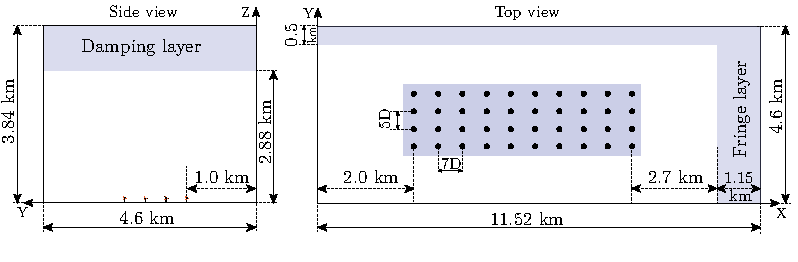
\includegraphics[width=\linewidth]{fig3}
 \caption{(a) Horizontally averaged wind magnitude $u_\mathsf{mag}/G$, (b) the vertical momentum flux, and (c) the temperature profiles plotted as a function of the height.}
 \label{fig3}
\end{figure}
\vspace{-5mm}
We consider a continuously turbulent, moderately stable ABL with a capping inversion at approximately 1000 m. The temperature similar to the one used in the Global Earth and Water Cycle Experiment (GEWEX) atmospheric boundary layer (GABLS) diurnal cycle, single column experiment\cite{kum10} with slight modifications. The boundary layer is initialized with a constant temperature of 286 $\mathsf{K}$ below 1000 $\mathsf{m}$, a capping inversion of strength 6 K/km between 1000 m and 1150 m, followed by a constant temperature gradient of 5 $\mathsf{K}\mathsf{km}^{-1}$ above. The roughness height, $z_o$ for momentum and heat are set to 0.002 m \cite{dor15} for off-shore conditions and 0.0002 m ($z_o/10$, \cite{bru82}), respectively. The surface is cooled at a constant rate of 0.5 K/hour. The geostrophic forcing is set to $G=(U_g,V_g)=(8.0,0.0)$ $\mathsf{m}\mathsf{s}^{-1}$ and the Coriolis parameter is set to $f_c=1.159\times10^{-4}$ $\mathsf{s}^{-1}$ corresponding to a latitude of $52.8^\circ$. The velocity is initialized with the geostrophic velocity. We note here that the boundary layer reaches a quasi-steady state at the end of 8$^\mathsf{th}$ hour.\\
%For stably stratified conditions, the ratio of the height of the first grid point to the roughness height, i.e.\ $z_1/z_o$, should be between 11 and 55 \cite{gar83, bas17}. If the first grid point is located lower the employed Monin-Obukhov similarity theory is namely not valid. Therefore, 
\indent The boundary layer characteristics relevant to this study are given in table \ref{table1}. The jet height $z_\mathsf{jet}$ is $125$ m and the ratio of boundary layer height to the surface Obukhov length $z_i/L=2.95$, which confirms that the boundary layer is moderately stable \cite{hol86}. Scaling regimes reported by \citeauthor{hol86} shows that for high $z_i/L > 5$, stable boundary layers show significant intermittency regime at the top of the boundary layer. For $z_i/L=2.95$ the intermittency regime is negligible, and LES can be safey used to study the SBL.\\
\indent LLJs of height approximately 80-150 m are often observed in the North Sea region of Europe \cite{baa09}. Figure \ref{fig3}(a) shows the horizontally averaged velocity magnitude $u_\mathsf{mag}=\left<\sqrt{\overline{u}^2+\overline{v}^2}\right>$ variation with height and Fig.\ \ref{fig3}(b) the corresponding horizontally averaged vertical turbulent momentum flux $\tau=\left<\sqrt{(\overline{u'w'})^2 + (\overline{v'w'})^2}\right>$, where $\overline{u'w'}=\left(\overline{{uw}} + \overline{\tau_{xz}}\right)-\overline{{u}}~\overline{{w}}$ and $\overline{v'w'}=\left(\overline{{vw}} + \overline{\tau_{yz}}\right)-\overline{{v}}~\overline{{w}}$. This figure reveals that there is negligible turbulence above the jet. Figure \ref{fig3}(c) presents the horizontally averaged potential temperature, which shows a strong surface inversion. The inversion height is defined as the height at which the temperature gradient is highest. The inversion top acts as a lid separating the turbulent and non-turbulent regions of the boundary layer.


\subsection{Computational domain and wind farm layout}\label{sec2.3} 
We consider a wind farm with 40 turbines distributed in 4 columns and 10 rows, see Fig.\ \ref{fig2}. We perform two sets of simulations, in the first set we keep the turbine diameter constant and change the hub height such that $z_h<z_{jet}$, $z_h\approx{z_{jet}}$, and $z_h>z_{jet}$, corresponding hub-heights are 60 m, 120 m, 180 m. The three cases represent the scenarios when the turbine rotor area is completely below the jet, distributed above and below the jet, and completely above the jet. We also performed an two additional simulations with a $z_h/D\approx0.75$ to understand how power varies under realistic $z_h/D$ ratios. In the second set of simulations the turbines are separated by $720$ m in the streamwise direction and $3D$ in the spanwise direction. 

The horizontal grid resolution is set to 9 m in both streamwise and spanwise directions. The computational domain is $11.52$ $\mathsf{km}$ $\times$ $4.6$ $\mathsf{km}$ $\times$ $3.84$ $\mathsf{km}$, which is discretized by $1280\times512\times384$ grid points. The grid points are uniformy distributed in the horizontal directions. We use uniformly distributed vertical grid points with a resolution of $5$ $\text{m}$ upto 1500 m and grid points are slowly stretched above. Here we emphasize that our simulations benefit from using an advanced Lagrangian dynamic sub-grid scale model, which has been shown to capture the dynamics of stable boundary layers very well. \cite{sto08, nag19}. Besides, we mention that Calaf et al.\ \cite{cal10} and Meyers and Meneveau \cite{mey13} showed that a resolution of $25$ m $\leq \Delta{x} \leq$ $50$ m in the streamwise direction and of $10$ m $\leq \Delta{y}\leq$ $25$ m in the spanwise direction is sufficient when an actuator disk method is used, while Wu and Port\'e-Agel \cite{wu11} showed that one needs $8$ points across the disk in the vertical direction and $5$ points in the spanwise direction. Clearly, our simulations satisfy these criteria as we use a $9$ m resolution in both the streamwise and spanwise direction, i.e.\ $9$ points in the spanwise direction and $16$ points in the vertical direction.



We choose turbines of $z_h/D\approx0.75$. Accordingly, the turbines have a diameter of $D=80$, $160$, and $240$ m. Corresponding, turbine hub heights are 60 m, 120 m, and 180 m are considered, which correspond to the cases where the turbine hub height is below the LLJ height ($z_h < z_\mathsf{jet}$), at the LLJ height ($z_h{\approx}z_\mathsf{jet}$), and well above the LLJ ($z_h > z_\mathsf{jet}$), respectively. We employ the concurrent precursor technique \cite{ste14} to introduce the inflow conditions sampled from the precursor simulation into the wind farm domain. Notably, we use fringe layers in both streamwise and spanwise directions to ensure that the wind veer is accurately represented in the wind farm domain.
A Rayleigh damping layer\cite{kle78} with a damping constant of 0.016 $\mathsf{s}^{-1}$ is used in the top 25$\%$ of the domain to damp out the gravity waves triggered by the wind farm. We use a proportional-integral (PI) controller\cite{all15} to ensure that the mean wind direction at hub-height is from West to East. The wind angle controller has been successfully used in our previous study of wind farms in neutral and stable boundary layers \cite{nag19} and ensures that the wind farm geometry is the same for all considered cases. The yaw misalignment due to the local changes in the wind angle is corrected by rotating the actuator disks such that the disks are always perpendicular to the local wind angle. Figure \ref{fig2} shows the wind farm layout and the dimensions of the different regions in the computational domain.

\begin{figure} 
 \centering
 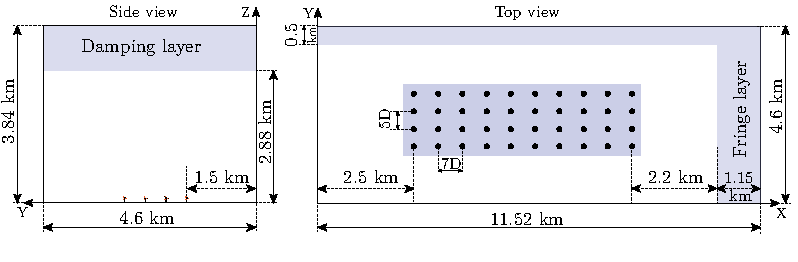
\includegraphics[width=\linewidth]{fig2}
 \vspace{-1.3cm}
 \caption{Schematic to show the wind farm layout with the damping layer to prevent gravity waves and the fringe layer that is used in the concurrent precursor method. The black circles denote the wind turbine locations. All the flow statistics are sampled from the shaded region with dimensions $70D\times{20D}\times{D}$ centered around the wind farm, see also figure \ref{cv}.}
 \label{fig2}
\end{figure}

%%%%%%%%%%%%%%%%%%%%%%%%%%%%%%%%%%%%%%%%%%%%
\section{Results \& discussions}\label{sec3}
The simulations were carried out in two stages. In the first stage, only the boundary layer in the precursor domain is simulated. After the quasi-steady conditions are reached, the turbines are introduced at the end of the 8$^\mathsf{th}$ hour. In this second stage, the simulations are continued for two more hours and the statistics are collected in the last hour. In section \ref{sec3.1} the flow structures are analyzed, followed by a discussion on power production, momentum flux, and wake recovery in section \ref{sec3.2}. In section \ref{sec3.3} an energy budget analysis is presented in which we discuss the diverse processes affecting the performance of the wind farm.

\subsection{Flow structures}\label{sec3.1}
\begin{figure}
 \centering
 \includegraphics[width=1.0\linewidth]{top_view}
 \caption{Normalized instantaneous velocity $u_\mathsf{mag}/G$ at hub-height for the three cases, i.e.\ (a) $z_h < z_\mathsf{jet}$, (b) $z_h \approx z_\mathsf{jet}$, and (c) $z_h > z_\mathsf{jet}$. Figs. (d), (e), and (f) present the corresponding time-averaged turbulence intensity, $\sigma_{u}/u_\mathsf{hub}$ where $\sigma_{u}=\sqrt{2k/3}$ and k is the turbulent kinetic energy. (g) Side view of the instantaneous streamwise velocity in an x-z plane through the second turbine column for the different cases.}
 \label{topview}
\end{figure}

A visualization of the instantaneous flow structures at hub-height is presented in Figs. \ref{topview}(a), (b), and (c). When $z_h<z_\mathsf{jet}$ (see Fig.\ \ref{topview}(a)), small scale structures are visible in the entrance region in front of the wind farm. In this case, the turbines operate in a completely turbulent region, and the wakes show significant mixing towards the end of the wind farm. Fig.\ \ref{topview}(b) shows that the turbulence intensity in the entrance region of the wind farm is low for the $z_h \approx z_\mathsf{jet}$ case. However, towards the rear of the wind farm sufficient turbulence is created by the wakes. When the turbines are above the jet (Fig.\ \ref{topview}(c)) there is limited turbulence at the entrance of the farm due to the strong thermal stratification in the negative shear region. However, after the first couple of rows the wakes have created significant turbulence. It is worth noting that for $z_h > z_\mathsf{jet}$ there is negligible lateral wake meandering behind the first turbine row and the wake recovery behind the first row is limited.

Figures \ref{topview}(d), (e), and (f) show the time-averaged turbulence intensity for all the three cases. The turbulence intensity is calculated as $\sigma_u=\sqrt{2k/3}$, where $k=0.5 (\overline{u'^2} +\overline{v'^2} + \overline{w'^2})$ is the resolved turbulent kinetic energy and $u_\mathsf{hub} = \sqrt{\overline{{u}}^2 + \overline{{v}}^2 + \overline{{w}}^2}$ is the velocity at the hub-height. When the turbines are below the LLJ (Fig.\ \ref{topview}(d)), the wakes recover relatively fast due to the high atmospheric turbulence and the additional wake added turbulence. In contrast, when $z_h \approx z_\mathsf{jet}$ and $z_h > z_\mathsf{jet}$ there is limited turbulence behind the first turbine row, especially for  $z_h > z_\mathsf{jet}$ when there is essentially no lateral wake meandering behind the first turbine row, see Fig.\ \ref{topview}(c). It is widely accepted that the turbine wake meandering is related to the atmospheric turbulence \cite{mao18, lar08} and in the absence of atmospheric turbulence the wake meandering is limited. Figure \ref{topview}(c) shows that the lateral wake meandering starts only behind the second turbine row when the turbines are above the LLJ. As a result, there is negligible turbulent kinetic energy behind the first turbine row (Fig.\ \ref{topview}(f)), which affects wake recovery of the wake behind the first turbine row and, therefore the power production of the second row.

Figure \ref{topview}(g) shows the side view of the wind farm in an x-z plane passing through the 2$^\mathsf{nd}$ turbine column. The top panel in Fig.\ \ref{topview}(g) shows the turbines operating in a turbulent region. The vertical entrainment caused by the turbines completely extracts the energy in the LLJ, which has also been observed in previous studies \cite{na18, lu11}. It is also worth noting that the turbine wakes show significant transverse meandering, which aids the extraction of momentum from the LLJ. When $z_h \approx z_\mathsf{jet}$, the turbines in the first row extract the energy in the jet and turbines operate in a well-mixed region after the second turbine row. Moreover, the LLJ is eliminated by the first turbine row, and therefore further downstream rows cannot benefit from the jet anymore. However, when $z_h > z_\mathsf{jet}$ the first couple of turbine rows are in a non-turbulent region, and therefore the turbulence after the first turbine row is limited. Furthermore, we observe no transverse wake meandering behind the first turbine row due to low atmospheric turbulence in the thermally stratified region above the jet. The strength of the jet is reduced towards the rear of the wind farm because of the transverse wake meandering and the positive entrainment flux generated by the wind turbine wakes, which will be discussed in detail in the next section.

%%%%%%%%%%%%% Sec 3.2 %%%%%%%%%%%%%%%%%%%%%%%%%%%%
\subsection{Power production and wake recovery}\label{sec3.2}
\begin{figure}
 \centering
 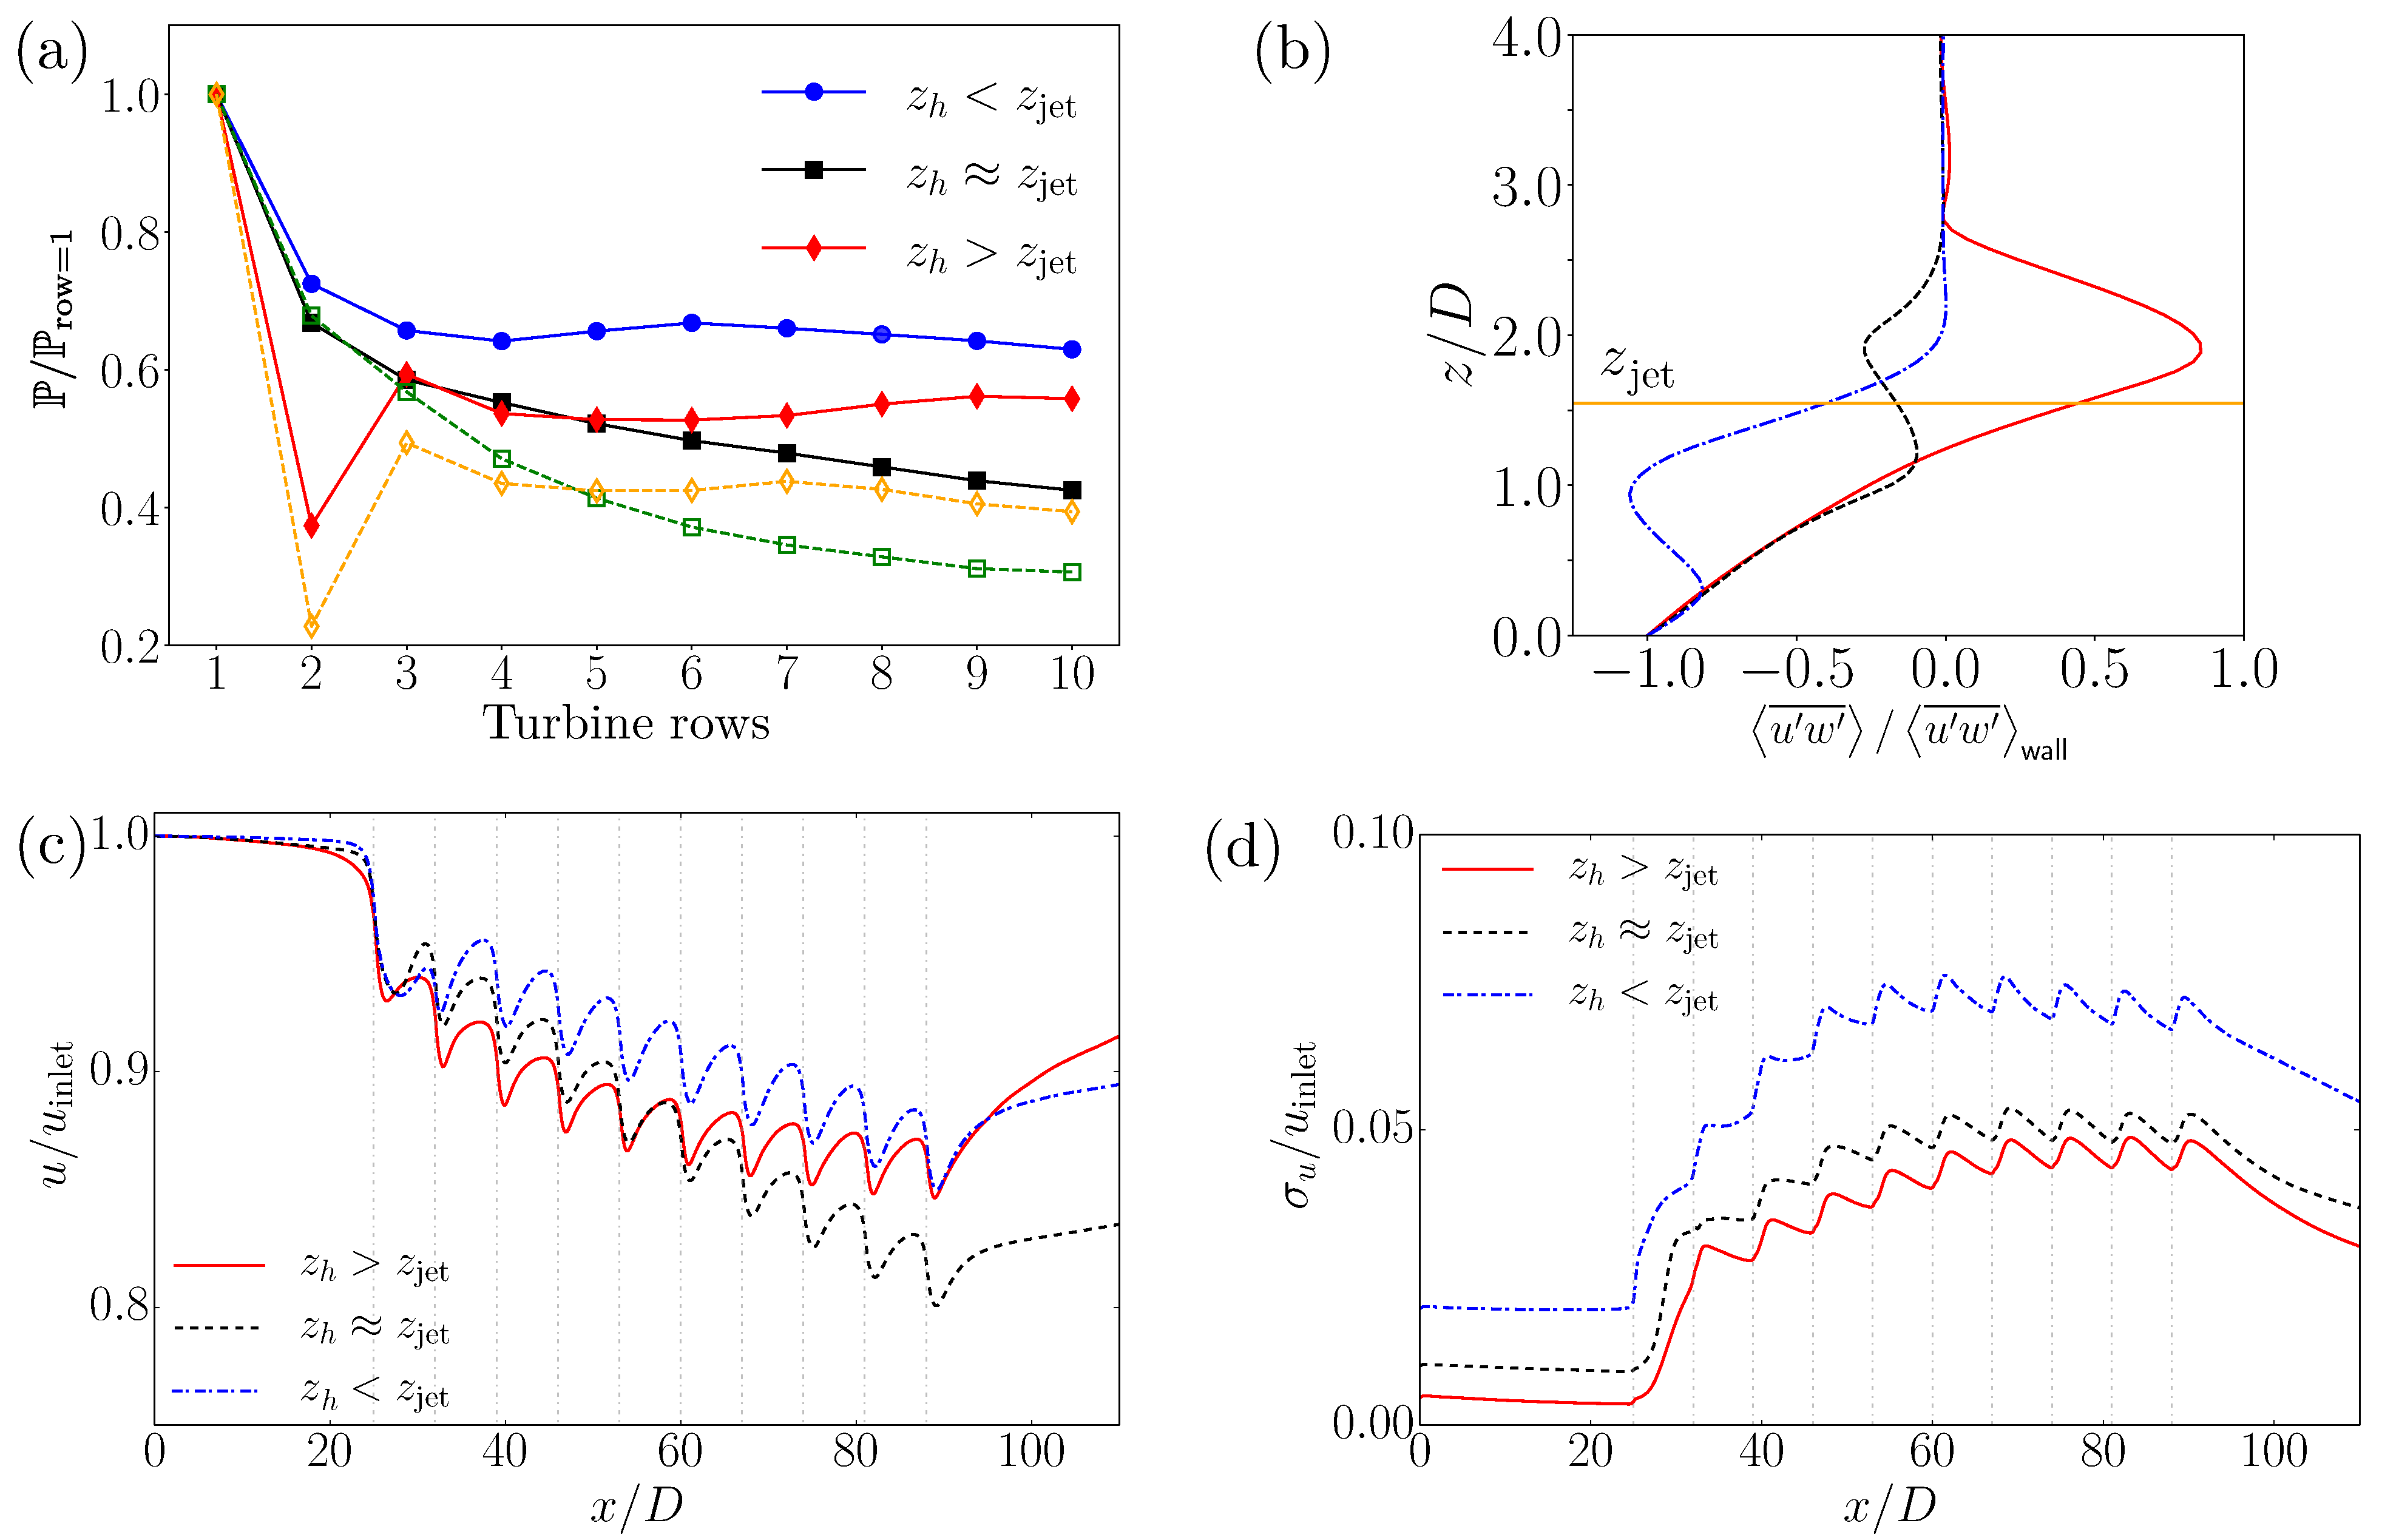
\includegraphics[width=0.9\linewidth]{powerplot_jrse} 
 \vspace{-0.25cm}
 \caption{(a) The row-averaged power normalized with the power production of the first row. The shaded region represents the standard deviation with respect to the mean. (b) Horizontally averaged streamwise vertical momentum flux versus height averaged over the wind farm domain. (c) Spanwise averaged streamwise velocity normalized with the upstream velocity at hub-height as a function of the streamwise location. (d) Streamwise variation of the turbulence intensity at hub-height for the three different cases.}
 \label{powerplots}
\end{figure}

The row-averaged power normalized by the power production of the first row is presented in Fig.\ \ref{powerplots}(a). The turbine power is averaged in the $10^\mathsf{th}$ hour of the simulation. To check the uncertainty in the power averaged over one hour, we collected the data as $10$-minute averages. The 10-minute averages are used to calculate the standard deviation of the one hour average, which is indicated in the figure. When $z_h < z_\mathsf{jet}$ we observe that the relative power production is higher further downstream, which means that velocity recovers faster than in the other cases, see Fig.\ 5(c). When $z_h \approx z_\mathsf{jet}$, the power production continuously reduces towards the rear of the wind farm, see Fig.\ \ref{powerplots}(a). The corresponding wake recovery shows that the velocity continuously drops in the downstream direction, which indicates that the wake recovery is negligible, see the dashed line in Fig.\ \ref{powerplots}(c). Interestingly, for the case with $z_h > z_\mathsf{jet}$, the power production of the second row is severely affected due to the absence of wake meandering in the wakes of the first row. However, as the wake meandering sets in, the power production increases, and it shows an upward trend towards the back of the wind farm. When $z_h > z_\mathsf{jet}$ the wake recovery improves after the wake meandering becomes dominant. Behind the second turbine row, when the wake meandering becomes significant for $x/D > 30$, the turbines entrain high momentum wind from the LLJ and the wake recovers significantly.

%%%%%%%%%%%%%%%%%%%%%%%%%%%%%%%%%%%%%%%%%%%

To better understand the wake recovery and the associated power variation, the vertical turbulent flux of streamwise momentum $\left<\overline{u'w'}\right>$ averaged over the wind farm domain and normalized by the $\left<\overline{u'w'}\right>$ at the wall are plotted in Fig.\ \ref{powerplots}(b). When $z_h < z_\mathsf{jet}$ there is a significant negative/downward momentum flux that is entrained from above, which extracts the jet's momentum and eliminates it towards the rear of the wind farm. However, for the cases $z_h \approx z_\mathsf{jet}$ and $z_h > z_\mathsf{jet}$ there is a significant positive entrainment flux. We observe in Fig.\ \ref{powerplots}(b) that for $z_h \approx z_\mathsf{jet}$ the momentum extraction by the wind farm creates a positive entrainment flux below and a negative entrainment flux above the jet. Consequently, the low-velocity wind below the jet continuously gets mixed, and this results in a continuous decrease of the power extraction by the turbines in the downstream direction as seen in Fig.\ \ref{powerplots}(a). Furthermore, the LLJ is eliminated by the first turbine row, which reduces the available flow energy for subsequent rows. However, when $z_h > z_\mathsf{jet}$, the turbines operate in the negative shear region of the jet, and the maximum positive flux is above the jet. As a result, the energy from the jet is entrained towards the hub-height plane and the power production shows an upward trend towards the end of the wind farm, see Fig.\ \ref{powerplots}(a). In essence, when the turbines interact with the negative shear region of the jet, the turbulence created by the wakes results in a significant positive turbulent flux. The jet's energy is entrained by the positive entrainment flux created by the negative shear, which enhances the wake recovery compared to the $z_h \approx z_\mathsf{jet}$ case.

For continuous production of turbulence $\overline{u'w'}\frac{\partial{\overline{u}}}{\partial{z}}$ should be negative. Therefore, in the presence of positive shear ($\frac{\partial{\overline{u}}}{\partial{z}}$ is positive) $\overline{u'w'}$ should be negative to produce turbulence. However, when the shear is negative ($\frac{\partial{\overline{u}}}{\partial{z}}$ is negative) $\overline{u'w'}$ should be positive to sustain turbulence. The tendency of the velocity deficit in the turbine wakes is to create a positive entrainment flux below the hub-height and a negative entrainment flux above hub-height. This leads to the following two scenarios: 
\begin{itemize}
 \item[1.] When $z_h < z_\mathsf{jet}$, the low momentum fluid below the hub-height mixes with high momentum fluid above the hub-height. As a result, we have a net downward entrainment flux, which is extracted by the turbines. The LLJ is eliminated due to this downward entrainment flux. 
 In this case, $\overline{u'w'}$ is negative and the horizontally averaged $\frac{\partial{\overline{u}}}{\partial{z}}$ is positive and there is a net negative vertical flux towards the hub-height.
 \item[2.] When $z_h > z_\mathsf{jet}$, the high momentum LLJ with a positive entrainment flux below the turbine hub-height mixes with the low momentum negative entrainment flux from above. The turbines extract the LLJ energy transported by the positive entrainment fluxes. 
 In this case, $\overline{u'w'}$ is positive and the horizontally averaged $\frac{\partial{\overline{u}}}{\partial{z}}$ is negative. The negative shear created by the turbine wakes increases the negative shear already present above the LLJ. As a result, there is a net positive vertical flux towards the hub-height. 
\end{itemize}

To quantify the turbulence produced by the wakes, the streamwise variation of the horizontally averaged turbulence intensity at the hub-height is plotted in Fig.\ \ref{powerplots}(d). When $z_h < z_\mathsf{jet}$, the turbulence intensity upstream of the farm is approximately 3.5\%, while it is approximately 0.9\% and 0.6\% for $z_h \approx {z_\mathsf{jet}}$ and $z_h > z_\mathsf{jet}$, respectively. We observe negligible wake meandering behind the first turbine row in Fig.\ \ref{topview}(d) when the turbines operate above the LLJ ($z_h > {z_\mathsf{jet}}$). After the wake meandering sets in behind the second turbine row the turbulence intensity increases and reaches values of approximately $6\%$ after the second row. It is clear from the above data that there is limited upstream turbulence when the turbines operate above the LLJ. Consequently, there is negligible wake recovery until the wakes generate enough turbulence. In essence, the negative shear in the jet creates a positive entrainment flux, which increases the turbulence intensity at hub-height. This accelerates the wake recovery and allows the turbines to extract energy from the jet. The turbulence intensity for the $z_h \approx {z_\mathsf{jet}}$ case develops in a very similar way as for the $z_h > {z_\mathsf{jet}}$ case as in both cases it is mostly determined by the wake added turbulence. However, when the turbines operate below the LLJ the turbulence intensity inside the wind farm is higher as the atmospheric turbulence interacts with the wind turbine wakes.

%%%%%%%%%%%%%%%% Sec 3.3 %%%%%%%%%%%%%%%%%%%%%%%
\subsection{Energy budget analysis}\label{sec3.3}
To understand the different processes involved in the power production of a wind farm in the presence of a LLJ we perform an energy budget analysis. The analysis is similar to the budget analysis performed by Allaerts and Meyers \citep{all17} for wind farms in conventionally neutral boundary layers. The steady-state, time-averaged energy equation is obtained by multiplying equation \ref{eqn2} with $\widetilde{u}_i$\cite{all17, sag06} and performing time-averaging, which results in:
\begin{equation}
\centering
\begin{split}
 \overbrace{\overline{u}_j\partial_j\left({\frac{1}{2}\overline{u}_i\overline{u}_i}+\frac{1}{2}\overline{u'_iu'_i}\right)}^\text{Kinetic energy flux}+\overbrace{\partial_j\left(\frac{1}{2}{\overline{u'_ju'_iu'_i}}+\overline{u}_i\overline{u'_iu'_j}\right)}^\text{ Turbulent transport}&+\overbrace{\partial_j\left( \overline{u_i\tau_{ij}}\right)}^\text{SGS transport}=\overbrace{-\partial_i{\left(\overline{pu_i}\right)}}^\text{Flow work}+\overbrace{g\beta(\overline{u_i\theta}-\overline{u}_i\theta_0)\delta_{i3}}^{\text{Buoyancy}}\\&+\overbrace{f_c\left(\overline{u}_iU_g\right)\delta_{i2}-f_c\left(\overline{u}_iV_g\right)\delta_{i1}}^{\text{Geostrophic forcing}}+\overbrace{\overline{f_iu_i}}^{\text{Turbine power}}+\overbrace{\overline{\tau_{ij}S_{ij}}}^{\text{Dissipation}}, 
\end{split} \label{eqn8} 
\end{equation}
where the time-averaging is represented by the overline, and $\overline{u'_iu'_j}=\left(\overline{{u_iu_j}}+\overline{\tau_\mathit{ij}}\right) - \overline{{u}_i}~\overline{{u}_j}$ indicates the momentum fluxes. To obtain the total power produced by each row we numerically integrate each term in equation \ref{eqn8} around a control volume surrounding each row. The control volume is chosen such that it encloses a row of wind farm, see Fig.\ \ref{cv}. Performing integration and rearranging equation \ref{eqn8} gives,
%Integral energy equation 
\begin{equation}
\centering
\begin{split}
 \overbrace{\int^{}_{\forall}\overline{f_iu_i}d\forall}^{\text{$\mathbb{P}$, Turbine power}}&=\overbrace{\int^{}_{\forall}\overline{u}_j\partial_j\left({\frac{1}{2}\overline{u}_i\overline{u}_i}+\frac{1}{2}\overline{u'_iu'_i}\right)d\forall}^\text{$\mathbb{E}_k$, Kinetic energy flux}+\overbrace{\int^{}_{\forall}\partial_j\left(\frac{1}{2}{\overline{u'_ju'_iu'_i}}+\overline{u}_i\overline{u'_iu'_j}\right)d\forall}^\text{$\mathbb{T}_\mathsf{t}$, Turbulent transport}+\overbrace{\int^{}_{\forall}\partial_j\left( \overline{u_i\tau_{ij}}\right)d\forall}^{\text{$\mathbb{T_\mathsf{sgs}}$, SGS transport}}+\overbrace{\int^{}_{\forall}\partial_i{\left(\overline{pu_i}\right)}d\forall}^{\text{$\mathbb{F}$, Flow work}}\\&-\overbrace{\int^{}_{\forall}g\beta(\overline{u_i\theta}-\overline{u}_i\theta_0)\delta_{i3}d\forall}^{\text{$\mathbb{B}$, Buoyancy}}-\overbrace{\int^{}_{\forall}f_c\left(\overline{u}_iU_g\right)\delta_{i2}-f_c\left(\overline{u}_iV_g\right)\delta_{i1}d\forall}^{\text{$\mathbb{G}$, Geostrophic 
 forcing}}-\overbrace{\int^{}_{\forall}\overline{\tau_{ij}S_{ij}}d\forall,}^{\text{$\mathbb{D}$, Dissipation}}
\end{split}\label{eqn9}
\end{equation}
where $\mathbb{P}$ is the power produced by a turbine row, $\mathbb{E}_k$ is the kinetic energy flux containing both resolved and SGS kinetic energy, $\mathbb{T}_t$ is the turbulent transport, which involves the transport of mean flow energy by turbulence \cite{lum72} and higher-order turbulence terms, $\mathbb{T}_\mathsf{sgs}$ is the mean energy transport by SGS stresses, $\mathbb{F}$ is the flow work, which is the pressure drop across the turbines, $\mathbb{B}$ is the turbulence destruction caused by buoyancy under stable stratification, $\mathbb{G}$ represents the geostrophic forcing driving the flow, and $\mathbb{D}$ is the SGS dissipation.

Figure \ref{energybudget}(a) and (b) present the energy budget analysis for cases with $z_h < z_\mathsf{jet}$ and $z_h > z_\mathsf{jet}$, respectively. All the terms are normalized by the absolute value of the power produced by the first turbine row. This normalization provides insight into the effect of wake recovery on power production. In both plots the energy sources are positive and sinks are negative. Both turbine power and dissipation act as energy sinks in the boundary layer. Fig.\ \ref{energybudget}(a) shows that for $z_h < z_\mathsf{jet}$ the kinetic energy $\mathbb{E}_k$ continuously decreases in the downstream direction. This reduction in the mean kinetic energy is compensated by the turbulent transport term $\mathbb{T}_t$. The turbulent transport slightly reduces after the fifth turbine row due to the elimination of the LLJ. In this case, the net downward entrainment of the fluxes compensates for the decrease in mean kinetic energy. In a fully developed wind farm boundary layer, the power production is completely balanced by the turbulent entrainment from above \cite{cal10, cal10b}. When the turbines operate in the positive shear region, the entrainment from above replenishes the energy extracted by the turbines. In addition to entrainment, the geostrophic forcing $\mathbb{G}$ and pressure drop $\mathbb{F}$ act as additional sources of energy. In contrast, turbulence destruction by buoyancy $\mathbb{B}$ and dissipation $\mathbb{D}$ remove energy from the control volume. When turbines are below the jet, i.e.\ $z_h < z_\mathsf{jet}$, there is positive shear in the boundary layer, due to which there is significant entrainment and wake recovery.

%%%%%%%%%%%%%%%
\begin{figure}
 \centering
 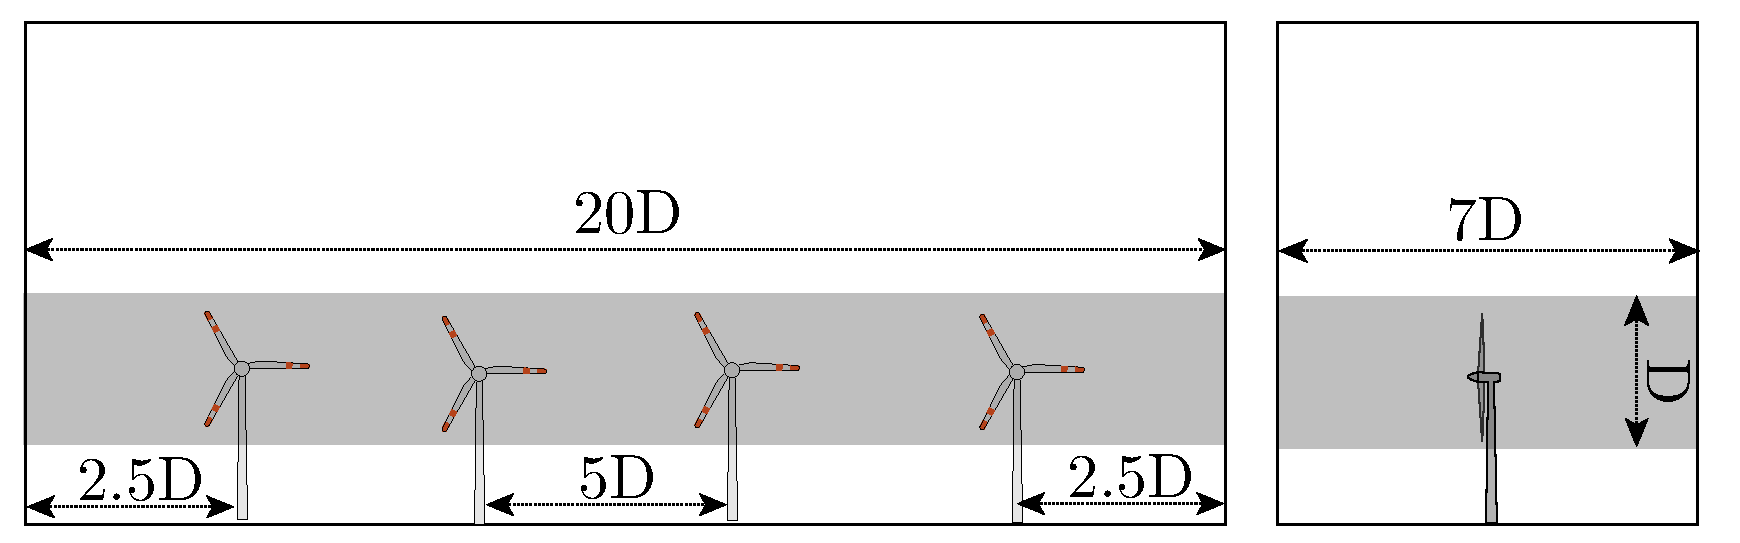
\includegraphics[width=0.75\linewidth]{controlvolume}
 \vspace{-0.25cm}
 \caption{The shaded region shows the control volume used in the energy budget analysis. The control volume around each turbine row has dimensions of $7\text{D}\times{20\text{D}}\times{\text{D}}$ in the streamwise, spanwise, and vertical directions, respectively. In the vertical direction the control volume starts at a height of $z_h-D/2$.}
 \label{cv}
\end{figure}

\begin{figure}[ht!]
 \centering
 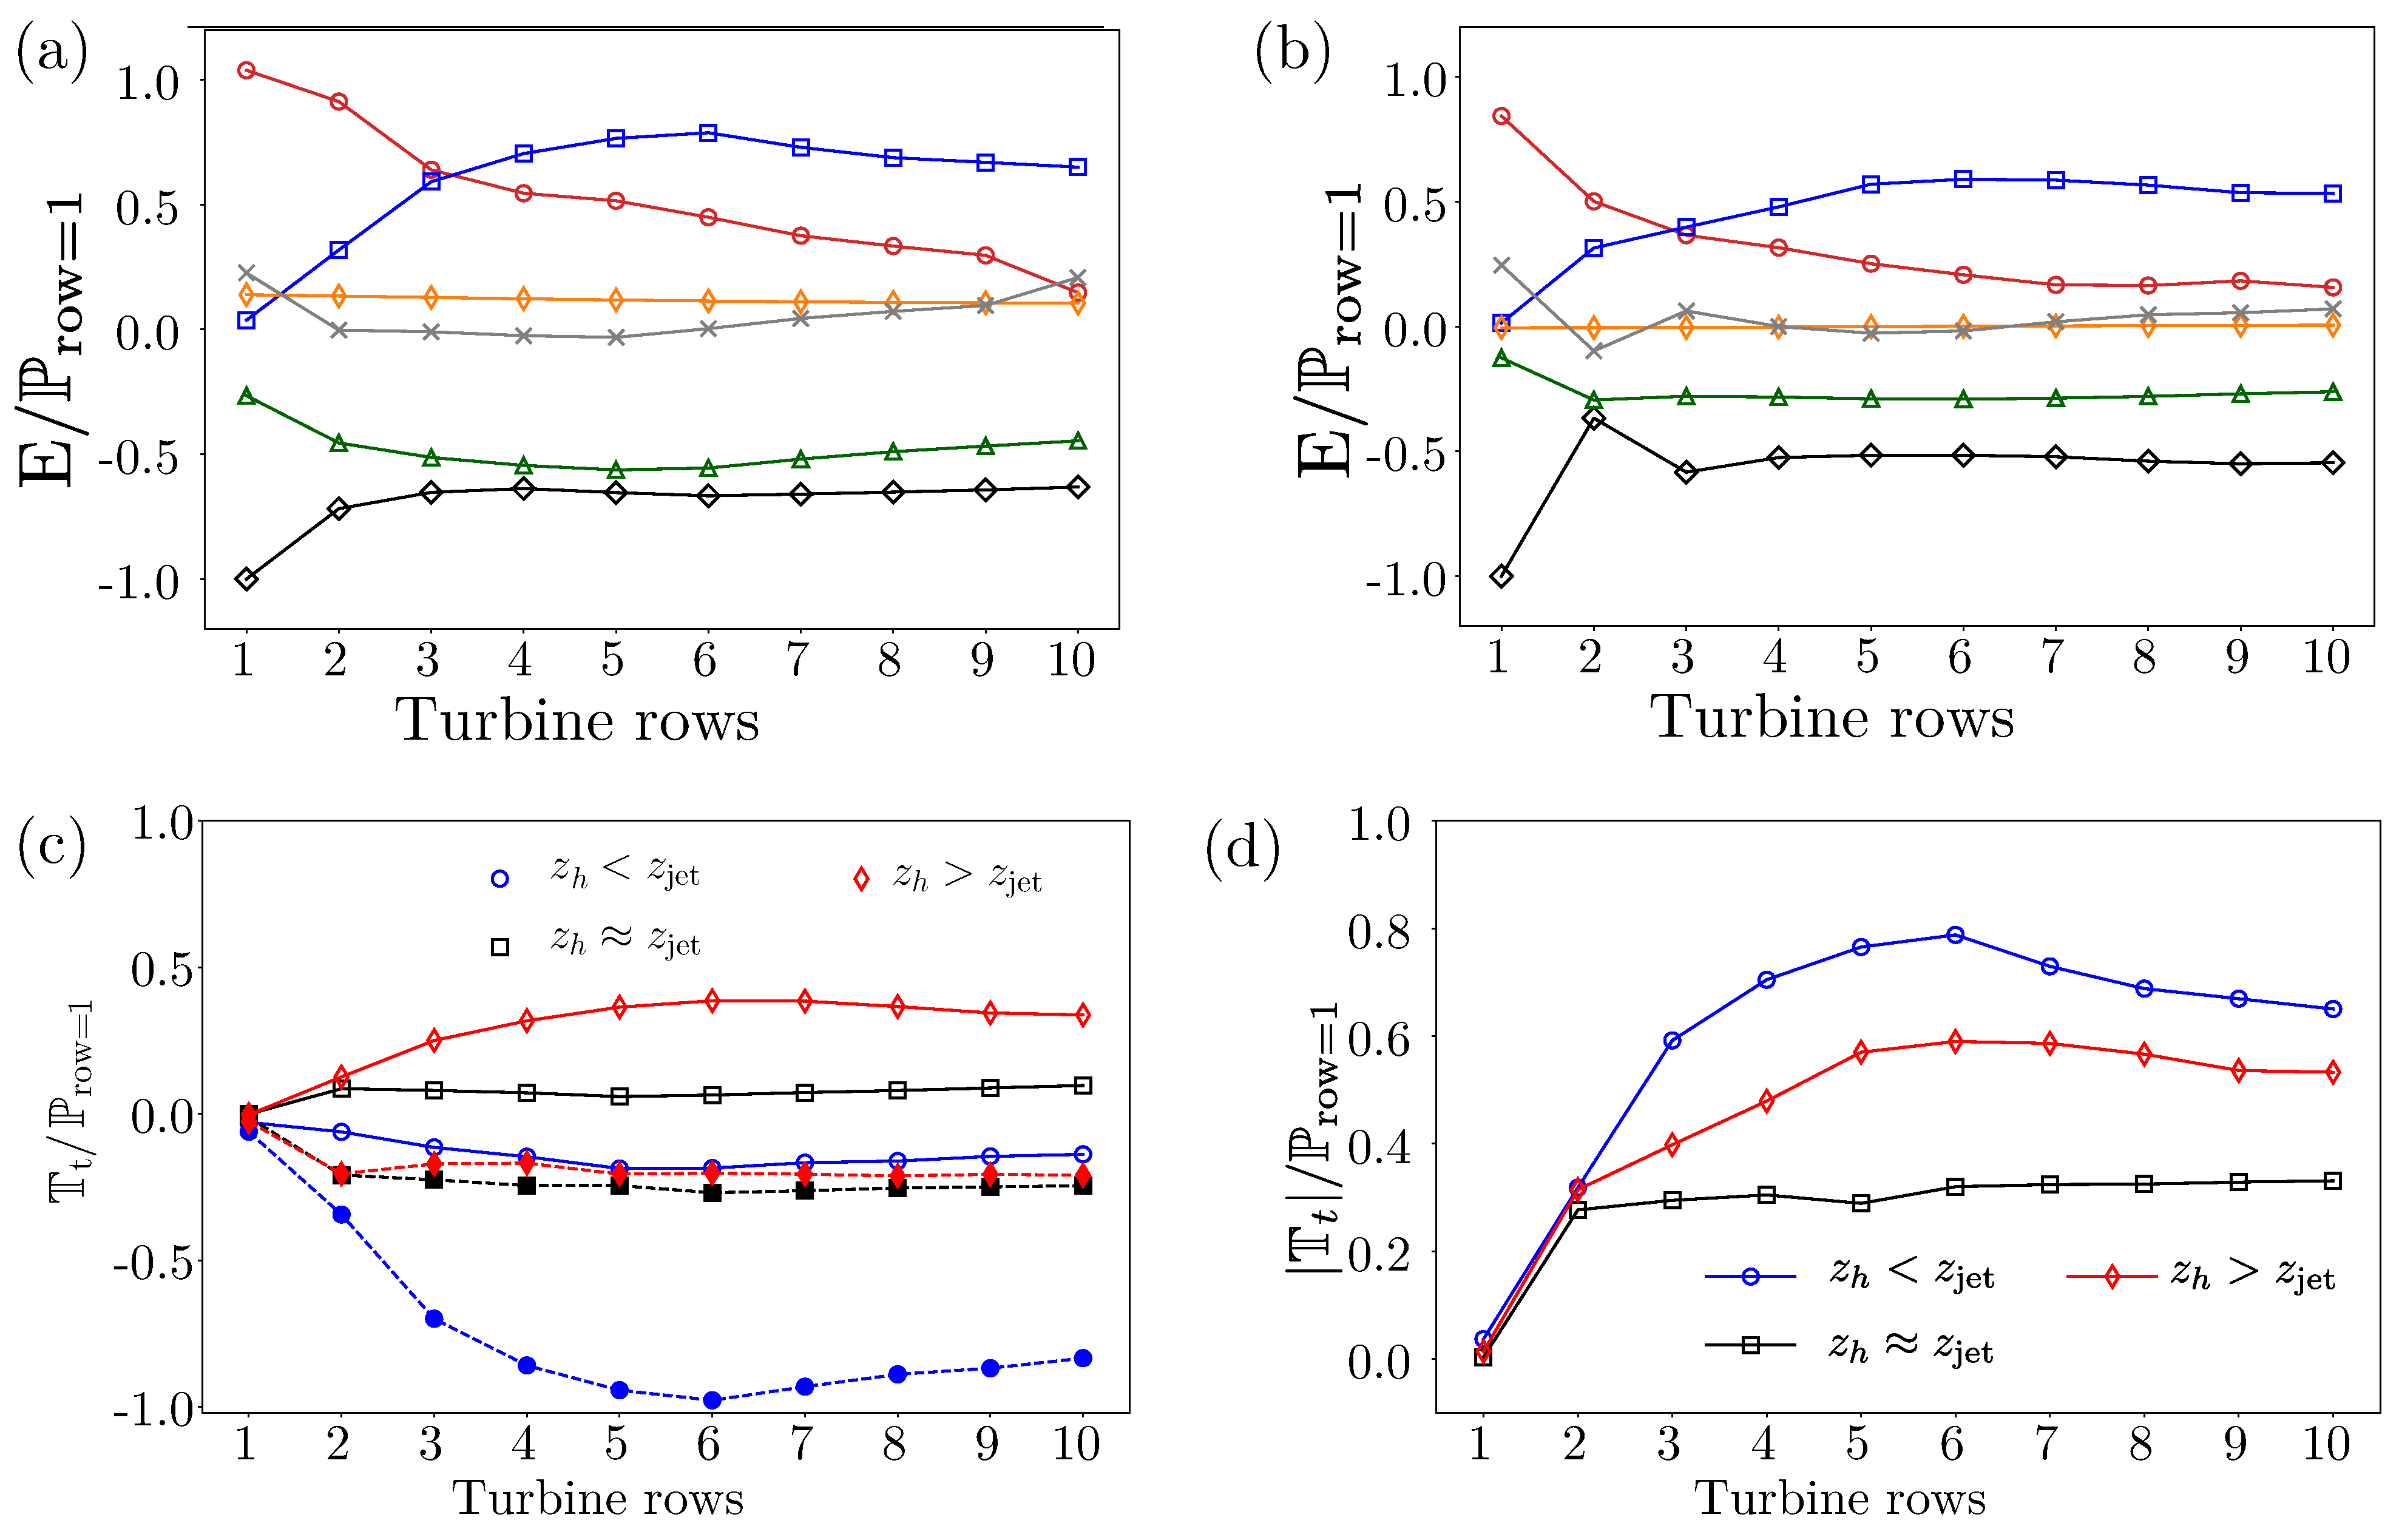
\includegraphics[width=0.9\linewidth]{energy_budget_jrse}
 \vspace{-0.75cm}
 \caption{Energy budget for (a) $z_h < z_\mathsf{jet}$ and (b) $z_h > z_\mathsf{jet}$. (c) Integrated entrainment flux over top and bottom planes of control volume. Dashes lines and solid symbols represent $\mathbb{T}_t$ on the bottom plane and solid lines \& filled symbols represent the heat flux on the top plane. (d) Net entrainment for different cases.}
 \label{energybudget}
\end{figure}

%%%%%%%%%%%%%%%%%%
When $z_h > z_\mathsf{jet}$ the kinetic energy $\mathbb{E}_k$ contribution drops after the first turbine row and recovers towards the third turbine row, the reason is the limited turbulence in the surrounding regions and the absence of wake meandering behind the first turbine row (Fig.\ \ref{energybudget}(b)) and there is negligible turbulent transport $\mathbb{T}_t$. The small turbulent transport $\mathbb{T}_t$ is entirely due to the turbulence generated by the wakes. The power production is mainly due to the mean flow energy extraction $\mathbb{E}_k$ and flow work $\mathbb{F}$. In essence, the wake recovery and the net entrainment due to turbulent transport are affected when the turbines are above the LLJ.

Figure \ref{energybudget}(c) provides a comparison of the turbulent transport term $\mathbb{T}_t$ for all the three cases. The figure shows that entrainment is strongest when $z_h < z_\mathsf{jet}$. The reason is that the boundary layer is turbulent below the jet, which aids the recovery of the turbine wakes. When $z_h \approx z_\mathsf{jet}$ the entrainment further downstream is affected as most of the energy from the jet is extracted by the first row. When $z_h > z_\mathsf{jet}$, there is increased entrainment due to the negative shear region of the jet, which creates a stronger turbulent transport $\mathbb{T}_t$ than for the $z_h=z_\mathsf{jet}$ case, but not as good as $z_h < z_\mathsf{jet}$.

\section{Conclusions}\label{sec4} 
We performed three LES of wind farms to study the effect of the turbine hub-height compared to the LLJ height on the interaction between with large wind farm, see Fig.\ \ref{fig1}. We considered three scenarios: 1) the turbine hub-height below the jet height, 2) the turbine hub-height equal to the jet height, and 3) the turbine hub-height above the jet height. When turbines operate below the jet the atmospheric turbulence adds to the turbine wake generated turbulence, which leads to a faster wake recovery. When the turbine hub-height is above the jet height, the turbines operate in a negative shear region of the LLJ, and the wake recovery is slower due to the limited atmospheric turbulence region above the LLJ. Furthermore, wake meandering plays a major role in wake recovery. In the absence of atmospheric turbulence the wakes are very stable \cite{mao18, kec14}. Due to the absence of atmospheric turbulence above the LLJ, the wakes created by the first turbine row do not meander, which adversely affects the power production of subsequent rows.

When the turbines are below the LLJ, the jet is eliminated due to the negative entrainment flux induced by the turbine energy extraction. When the turbine hub-height is equal to the jet height, the energy in the jet is extracted by the first turbine row and the rest of the rows do not benefit from the jet. When the turbines are above the jet the mean negative shear and the shear created by the wakes create a net positive vertical flux towards the hub-height. This {\color{black} negative shear aids in the extraction} of the energy from the jet. Although the negative shear above the LLJ creates a positive turbulent entrainment flux the turbulence production it creates is limited due to the thermal stratification above the jet.

The energy budget analysis reveals that the vertical entrainment dominates the power production when the turbines are below the LLJ. In contrast, the pressure drop and mean kinetic energy drop are the major contributors to power production when the turbines are above the jet. The relative power production of the turbines further downstream in the wind farm depends on the position of the jet relative to the hub-height. {\color{black} Relative power production of the turbines with hub-height lower than the jet-height is higher than the turbines with hub-height above the jet-height. This is due to the higher turbulence intensity in the region below the jet compared to the region above the jet where the turbulence is negligible due to the surface inversion.}

Gutierrez et al.\ \cite{gut17} report the reduction in the turbine loads due to the negative shear in the LLJ and therefore suggest installing turbines such that they are in this region. However, here we show that the reduction in the power production of downstream rows due to slower wake recovery may offset the structural stability advances. Here we emphasize again that we used the LLJ from the GABLS-1 moderately stable benchmark case to study the general physical phenomena that result from the interaction of a LLJ with a large wind farm. However, further work will be required to investigate the effect of higher thermal stratification, complex terrain, the strength of the geostrophic wind and its direction, the transition from land to sea on the LLJ characteristics, and how this affects the performance of wind farms.

\section*{author's contributions}
\noindent All authors contributed equally to the manuscript.  

\begin{acknowledgments}
This work is part of the Shell-NWO/FOM-initiative Computational sciences for energy research of Shell and Chemical Sciences, Earth and Live Sciences, Physical Sciences, FOM, and STW. This work was carried out on the national e-infrastructure of SURFsara, a subsidiary of SURF corporation, the collaborative ICT organization for Dutch education and research and an STW VIDI grant (No. 14868).
\end{acknowledgments}

\section*{Data availability}
\noindent The data that support the findings of this study are available from the corresponding author upon reasonable request.

%\section*{Appendix}
%In figure \ref{fig:grid} we show that the velocity (figure \ref{fig:grid}(a)) and temperature (figure \ref{fig:grid}(b)) profiles obtained in our simulations agree well with the very high-resolution results presented by Beare et al.\ \cite{bea06}. The comparison of the surface layer similarity with the observations of Nieuwstadt \cite{nie84} are presented in figure \ref{fig:grid}(c). In agreement with Beare et al.\ \cite{bea06} we find that our results on the locally-scaled non-dimensional shear agree with the Nieuwstadt \cite{nie84} observations and show a z-less stratification regime for $z/\Lambda > 2.0$. The vertical momentum flux, which is important to calculate the boundary layer height, is presented in figure \ref{fig:grid} and also matches the Beare et al.\ \cite{bea06} results well. The figure also shows the results obtained on three different grid resolutions and confirms that the result obtained on the grid used in this study ($9$ m $\times9$ m $\times5$ m) ensures that the boundary layer dynamics are captured appropriately.

%\begin{figure}[h!]
% \centering
% 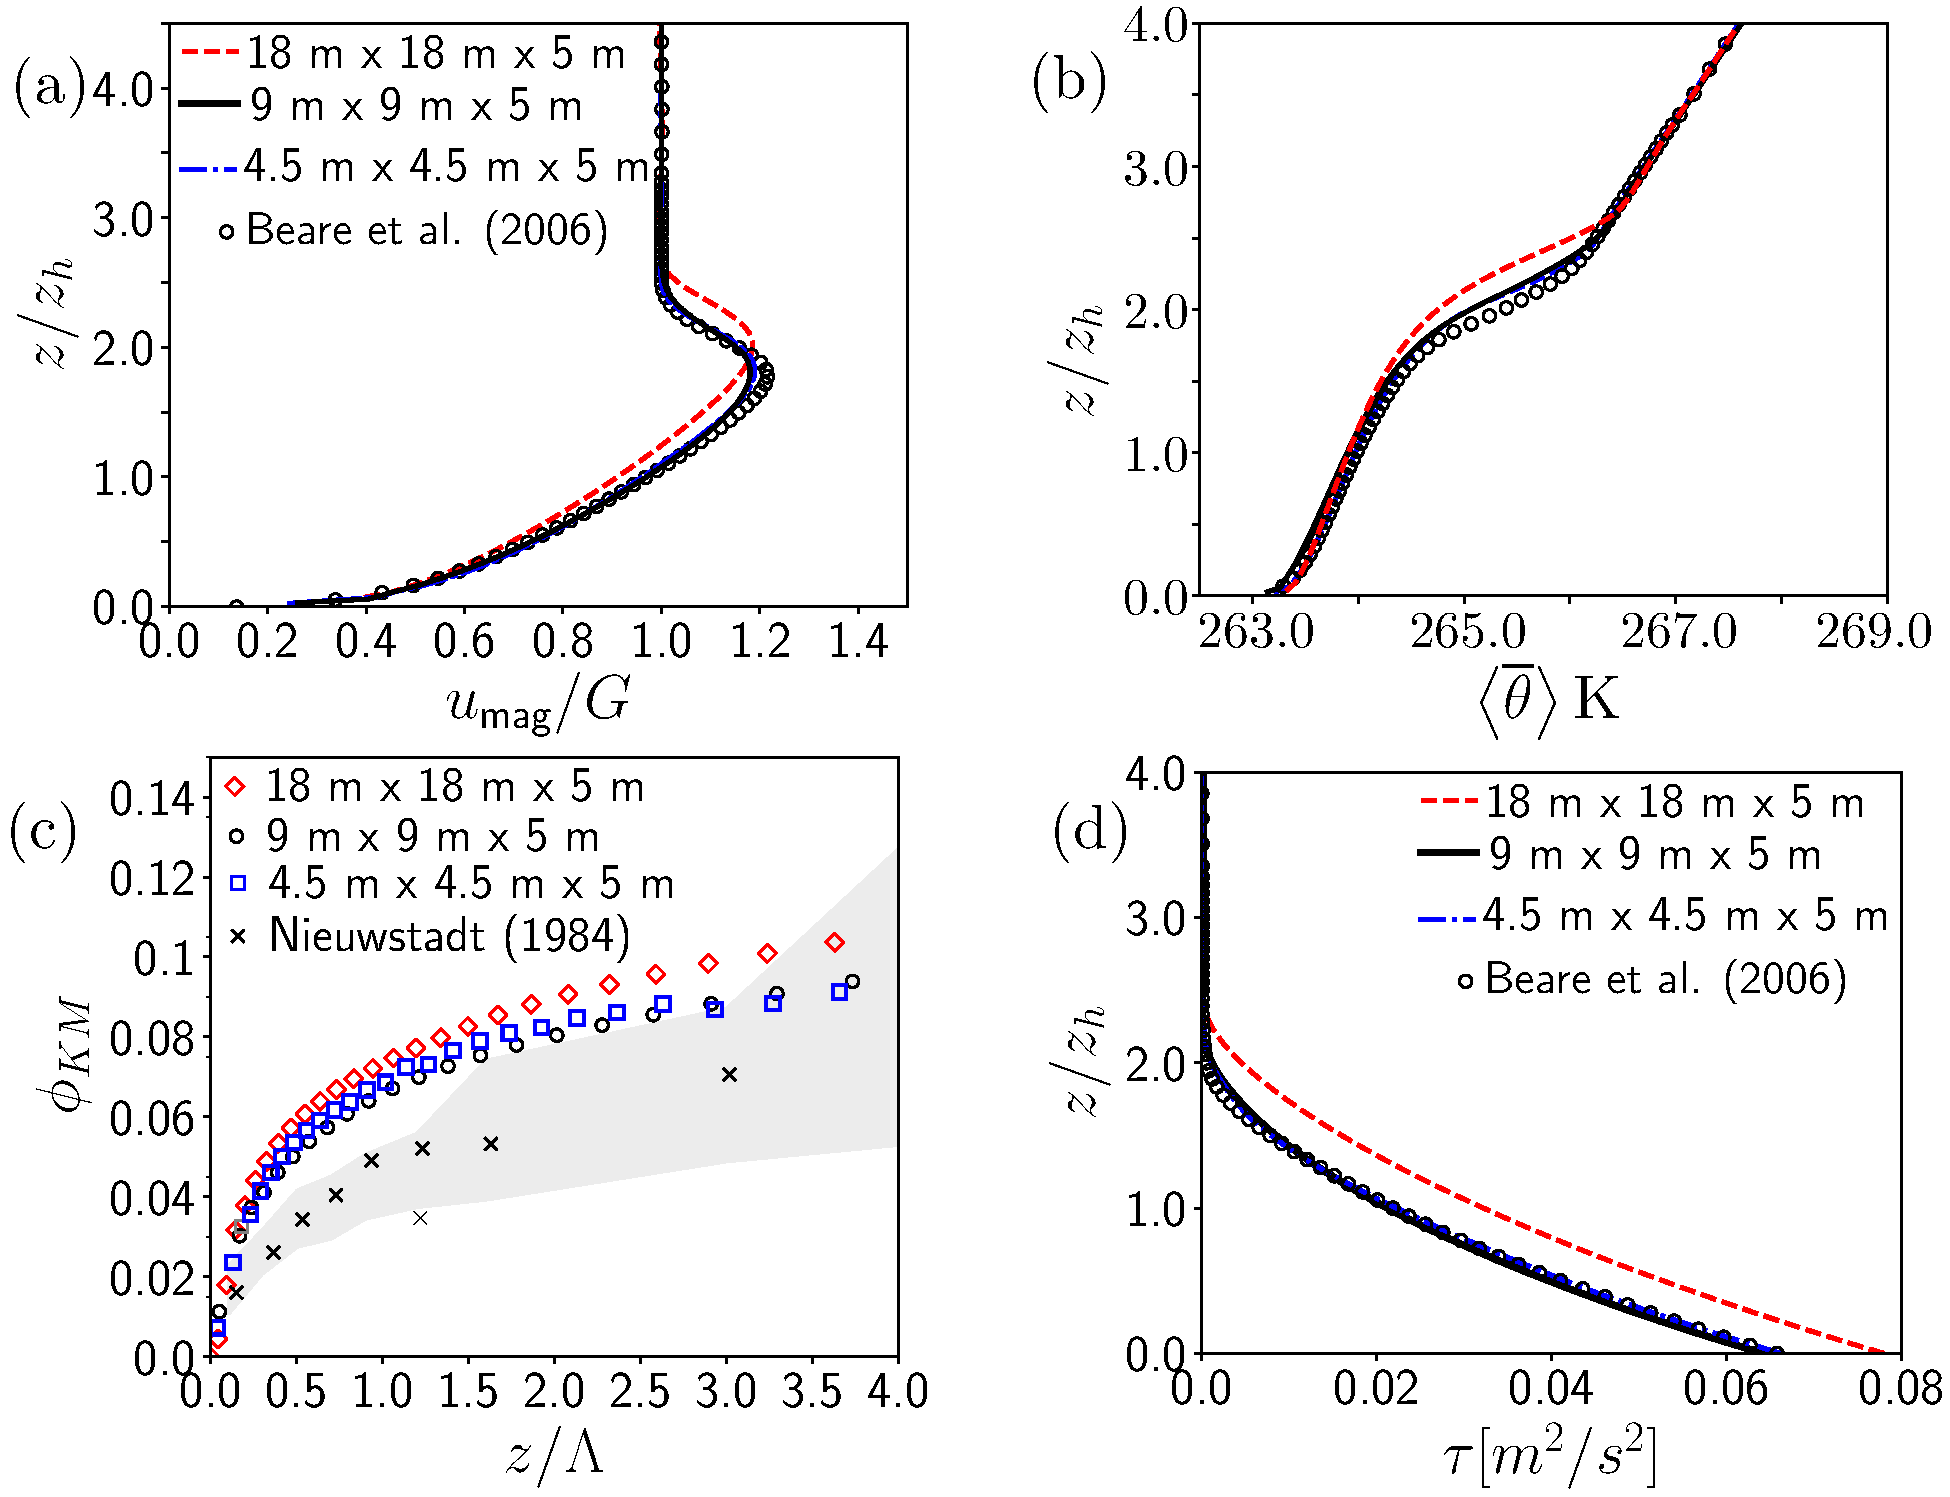
\includegraphics[width=0.8\textwidth]{grid_independence_final.pdf}
% \vspace{-0.4cm}
% \caption{Validation of our simulations against the Beare et al.\cite{bea06} results. (a) Velocity magnitude. (b) Potential temperature. (c) Non-dimensional shear plotted against locally scaled Obukhov length $\Lambda$. The shaded region represents the spread in the data of the Nieuwstadt (1984) \cite{nie84} observations. (d) Vertical momentum flux.}
% \label{fig:grid}
%\end{figure}


\bibliography{literature_windfarms}


\end{document}
